%!TEX TS-program = xelatex
\documentclass[]{friggeri-cv}
\usepackage{afterpage}
\usepackage{hyperref}
\usepackage{color}
\usepackage{xcolor}
\usepackage{smartdiagram}
\usepackage{fontspec}
\usepackage{graphicx}
\usepackage{subcaption}


% if you want to add fontawesome package
% you need to compile the tex file with LuaLaTeX
% References:
%   http://texdoc.net/texmf-dist/doc/latex/fontawesome/fontawesome.pdf
%   https://www.ctan.org/tex-archive/fonts/fontawesome?lang=en
%\usepackage{fontawesome}
\usepackage{metalogo}
\usepackage{dtklogos}
\usepackage[utf8]{inputenc}
\usepackage{tikz}
\usetikzlibrary{mindmap,shadows}
\hypersetup{
    pdftitle={},
    pdfauthor={},
    pdfsubject={},
    pdfkeywords={},
    colorlinks=false,           % no lik border color
    allbordercolors=white       % white border color for all
}
\smartdiagramset{
    bubble center node font = \footnotesize,
    bubble node font = \footnotesize,
    % specifies the minimum size of the bubble center node
    bubble center node size = 0.5cm,
    %  specifies the minimum size of the bubbles
    bubble node size = 0.4cm,
    % specifies which is the distance among the bubble center node and the other bubbles
    distance center/other bubbles = 0.29cm,
    % sets the distance from the text to the border of the bubble center node
    distance text center bubble = 0.28cm,
    % set center bubble color
    bubble center node color = pblue,
    % define the list of colors usable in the diagram
    set color list = {lightgray, materialcyan, orange, green, materialorange, materialteal, materialamber, materialindigo, materialgreen, materiallime},
    % sets the opacity at which the bubbles are shown
    bubble fill opacity = 0.6,
    % sets the opacity at which the bubble text is shown
    bubble text opacity = 0.5,
}

\addbibresource{bibliography.bib}
\RequirePackage{xcolor}
\definecolor{pblue}{HTML}{0395DE}

\begin{document}
\header{SiThu}{Thwin}
      {SRE Team Lead and Solution Architect}

% Fake text to add separator
\fcolorbox{white}{gray}{\parbox{\dimexpr\textwidth-2\fboxsep-2\fboxrule}{%
.....
}}
%...

% Add badges
\begin{figure}[h]
  \centering
  \begin{subfigure}[b]{0.1\linewidth}
    
\includegraphics[width=\linewidth]{img/cka.png}
  \end{subfigure}
  \begin{subfigure}[b]{0.1\linewidth}
    
\includegraphics[width=\linewidth]{img/istio-expert.png}
  \end{subfigure}
  \begin{subfigure}[b]{0.1\linewidth}
    
\includegraphics[width=\linewidth]{img/istio-intermediate.png}
  \end{subfigure}
  \begin{subfigure}[b]{0.1\linewidth}
    
\includegraphics[width=\linewidth]{img/istio-fundamentals.png}
  \end{subfigure}
  \begin{subfigure}[b]{0.1\linewidth}
    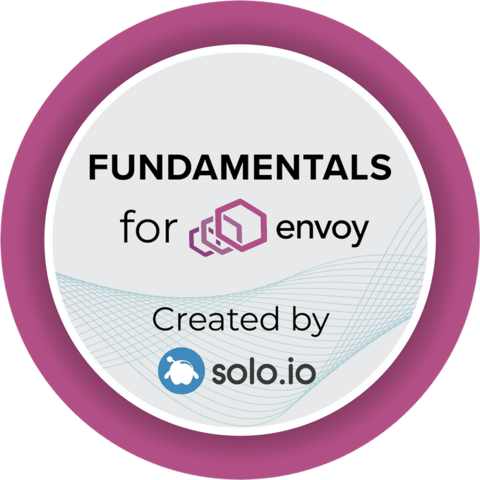
\includegraphics[width=\linewidth]{img/envoy.png}
  \end{subfigure}
  \begin{subfigure}[b]{0.1\linewidth}
    
\includegraphics[width=\linewidth]{img/ccna.png}
  \end{subfigure}
\end{figure}
%...

% In the aside, each new line forces a line break
\begin{aside}
  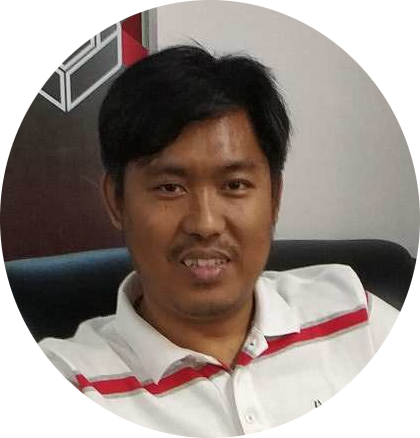
\includegraphics[scale=1]{img/myself-circle.png}
  \section{Address}
    CL1-202, Cityloft@Starcity
    Than Lyin Township
    Yangon, Myanmar
    ~
  \section{Contact}
    \textbf{Tel:} +95 979 7969695
    \textbf{Skype:} live:sithuthwin
    ~
  \section{Mail}
    \href{mailto:sithu@thwin.net}{\textbf{sithu@}thwin.net}
    ~
  \section{Social}
    \textbf{LinkedIn:} \href{https://www.linkedin.com/in/si-thu-thwin/}{si-thu-thwin}
    ~
  \section{Web \& Git}
    \href{https://www.thwin.net}{thwin.net}
    \href{https://github.com/herzcthu}{github.com/herzcthu}
    \href{https://gitlab.com/herzcthu}{gitlab.com/herzcthu}
    ~
  % use  \hspace{} or \vspace{} to change bubble size, if needed
  \section{DevSecOps}
    \textbf{GitLab CI/CD}
    \textbf{Terraform/Ansible}
    \textbf{SonarQube}
    \textbf{Maven}
    \textbf{Docker}
    \textbf{ELK/EFK}
    \textbf{Prometheus/Grafana}
    \textbf{K8S/Openshift/Helm/Istio/Single Mesh}
    \textbf{Pinpoint/Zipkin}
    \textbf{PHP}
    \textbf{Python/Flask}
    \textbf{YAML}
    \textbf{Bash}
    \textbf{LaTeX}
    \textbf{gRPC/mTLS/PKI}
    \textbf{AWS/Azure/Oracle}
    \textbf{MySQL/MongoDB}
    ~
\end{aside}
~
%...

\section{Skills}
\begin{entrylist}
  \entry
  {Mesh}
  {Kubernetes, ISTIO, Helm, Single Mesh, Service Discovery}
  {DevOps}
  {  \begin{itemize}
      \item More than 4 year experiences working with Kubernetes and Istio.
      \item Setup and maintain multi datacenter, multi cluster single mesh and service discovery using ISTIO.
      \item Well experienced working with ISTIO ingress gateway, virtual services, mTLS and istio API resources.
      \item Very well understanding about Kubernetes APIs and resources. Very well experienced creating helm charts.
      \item Very well experienced working with stateful apps and statefulset in Kubernetes. Very well experienced working with Kubernetes operators.
    \end{itemize}}
  \entry
  {Messaging}
  {Kafka, ActiveMQ, Strimzi, Debezium}
  {DevOps}
  { \begin{itemize}
      \item Deploy, manage and maintain Kafka Cluster on Kubernetes and VM. 
      \item Deploy, manage and maintain Debezium for CDC.
      \item Manage Strimzi Operator for Kafka Cluster. Deploy and manage ActiveMQ on Kubernetes and VM.
    \end{itemize}}
  \entry
  {GitOps}
  {GitOps, GitFlow, Gitlab}
  {DevOps}
  { \begin{itemize}
      \item Well experienced on git operation. Well established knowledge on git and gitflow.
      \item Organize repositories for easier management (Current organization follow the SOP created by myself)
    \end{itemize}}
  \entry
  {Pipeline}
  {Gitlab Pipeline, Jira Integration, MS Team Integration}
  {DevOps}
  { \begin{itemize}
      \item Creating pipeline on gitlab. I can work on any other pipeline tools.
      \item Integrate with any agile tools or communication channels
    \end{itemize}}
  \entry
  {Database}
  {Oracle, MySQL, MongoDB, SQL}
  {DBA}
  { \begin{itemize}
      \item Very proficient with SQL queries
      \item Basic understanding about Oracle RAC cluster, RMAN, Dataguard
      \item Well understanding about MongoDB cluster and can manage the cluster
      \item Well understanding about MySQL server, clusters and replication
    \end{itemize}}
  \entry
  {APM}
  {Grafana, Prometheus, Jaeger, Zabbix, Pinpoint, Graylog}
  {DevOps}
  { \begin{itemize}
      \item Proficient with setting up various montoring tools
      \item Very good experiences with pinpoint APM
      \item Graylog or ELK stack
    \end{itemize}}
\end{entrylist}
\newpage
~

\begin{aside}
  ~
  ~
  ~
  ~
  \section{Referee}
  \textbf{Sander Meinema}
  \href{mailto:sander@architectingasaservice.com}{\textbf{sander@}architectingasaservice.com}
\end{aside}
\section{Experience}
~

\begin{entrylist}
  \entry
    {08/20 - Now}
    {SRE team Lead and Solution Architect}
    {YOMA Bank}
    {Lead and Manage DevOps team and SRE team, VMWare, System Team, DBA Team and ApplicationRelease team combined as future SRE team which include more than 20 engineers.\\Design CI/CD pipeline architecture that include centralized configuration management to use in the whole organization.\\Create gitflow principles to be followed by all developers and DevOps.\\Solution Architect for personal banking, next generation mobile banking, business credit card portal and bancassurence.\\Create microservices architecture principles for the whole organization.\\Create API GW integration architecture principles\\Design and build essential microservices to use in various integration.\\Lead CBMNet-II integration development\\Conducted various training of technologies related with DevSecOps for engineers in the organization}
  \entry
    {03/19 - 08/20}
    {Lead DevOps Engineer}
    {YOMA Bank}
    {Lead DevOps in Digital Transformation. Designed CI/CD pipeline and Gitflow for new mobile/online banking app based on Backbase.\\Deploy Kubernetes Cluster on Azure and on-premise Datacenter.\\Integrate ISTIO and Netflix Eureka based microservices.\\Develop k8s helm charts for backbase deployment.\\Maintain maven files for JAVA package and docker image building.\\Training DevOps team.\\Work closely with Backbase Solution Team for deployment and infrastructure architecture.\\Build scalable deployment for Backbase framework and related system such as ActiveMQ.\\Successfully integrate ISTIO with Backbase to use all essential features in ISTIO such as mTLS. Probably I'm the first person in the world to do this in production system.\\}
  \entry
    {11/17 - 03/19}
    {Assistant Team Lead (System and Database)}
    {YOMA Bank}
    {Oracle and MySql management. Maintain Digital Channel (Mobile Banking) and Finastra's Fusion Middleware\\
    }
  \entry
    {08/17 - 11/17}
    {Database Specialist}
    {YOMA Bank}
    {Oracle and MySql management. Developed Cash Management Portal (YOMA and McKinsey project)\\}
  \entry
    {04/16 - 08/17}
    {Senior System Administrator}
    {Blue Ocean Call Center}
    {Manage SIP Gateway, Asterisk, VMware, UCS server, SIP routing.\\ Lead and completed to setup call center for Grab Taxi Myanmar.\\ Developed CRM for CocaCola Myanmar\\ }
    ~
\end{entrylist}
\newpage
~

\section{Other Experiences and Professions}
~
\begin{entrylist}
  \entry
  {Trainer}
  {Trainer for DevSecOps Engineering}
  {BIM Training}
  {Teach and train for DevSecOps Engineering classes}
  \entry
  {Mentorship}
  {Mentor for CS50}
  {Personal}
  {Personal mentor for CS50 - Introduction to computer science}
  \entry
  {Consultant}
  {ICT Consultant for Election Monitoring}
  {NDI, Washinton DC}
  {Develop data collection software (Web based and SMS). Data syncronization between cloud and local server. This software is used in 
    \begin{itemize}
      \item 2015 General Election Myanmar
      \item 2017 By-Election Myanmar
      \item 2017 General Election Cambodia
      \item 2020 General Election Myanmar
    \end{itemize}}
  \entry
  {Cloud}
  {DataCenter Migration}
  {blueplanet.com.mm}
  {Move on-prem datacenter to AWS cloud. Auto scaling EC2 instances using spot instance. Data replication between on-prem and cloud. Asterisk SIP routing from cloud to on-prem servers.\\}
\end{entrylist}
\section{Education}
\begin{entrylist}
  \entry
    {2001 - 2004}
    {Bachelor's Degree in German Language}
    {UFL, Mandalay}
    {Specialized in German Language\\ }
\end{entrylist}


\begin{aside}
~
~
~
~
  \section{Personal Skills}
  \smartdiagram[bubble diagram]{
    \textbf{Quick}\\\textbf{Learner},
    \textbf{Organize},
    \textbf{Team}\\\textbf{Player},
    \textbf{Initiative},
    \textbf{Curiosity},
    \textbf{Problem}\\\textbf{Solving},
    \textbf{Manage}
  }
~
\end{aside}
\section{Certifications}
\begin{entrylist}
  \entry
  {01/2023}
  {CKA}
  {cncf.io}
  {\emph{Certified Kubernetes Administrator}}
  \entry
  {04/2019}
  {LinuxFoundationX - LFS158x}
  {edx.org}
  {\emph{Introduction to Kubernetes}}
  \entry
  {09/2014}
  {CCNA Cisco Certified Network Associate}
  {PearsonVUE}
  {\emph{Routing and Switching}}
\end{entrylist}

\section{Training}
\begin{entrylist}
  \entry
  {Self-Paced}
  {LFS258 Kubernetes Fundamentals}
  {linuxfoundation.org}
  {Certified Kubernetes Administrator Program}
  \entry
  {09/2018}
  {RedHat Openshift Workshop}
  {RedHat}
  {\emph{Openshift setup on-prem with Ansible. Openshift Architecture}}	\entry
  {07/2018}
  {VMware Certified Professional 6.5}
  {BIM Training, VMware Official}
  {\emph{Datacenter Virtualization}}
  \entry
  {09/2014}
  {Advanced Network Engineering}
  {RHC Technologies}
  {\emph{Advanced networking. Routing and switching}}
\end{entrylist}

\textbf{\emph{March 20th, 2023}}
\hfill
\textbf{\emph{Sithu Thwin}}
\end{document}